\section{Architecture} % (fold)
\label{sec:architecture}
Figure \ref{fig:dependencygraph} shows the most essential parts of the internal MiCS architecture and how the parts depend on each other. 
This section will describe the different parts, how they relate to one another and how the architecture relates to the five stages outlined in section \ref{sec:workflow_overview}. 

\begin{figure}
	\begin{center}
		\centerline{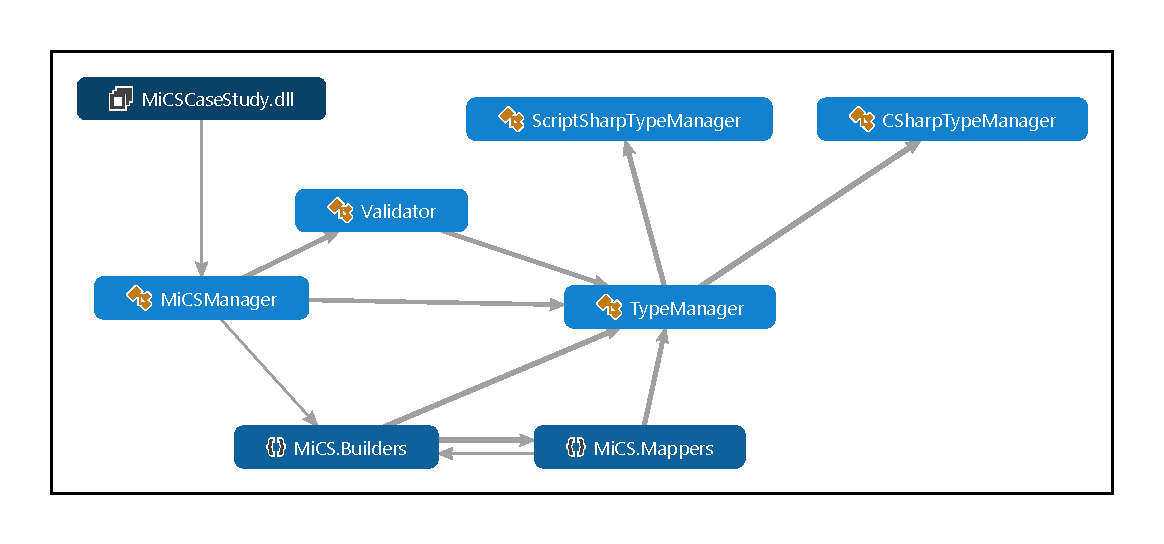
\includegraphics[width=18cm]{resources/images/dependencygraph.pdf}}
	\end{center}
	\caption{The most important parts of the MiCS architecture}
	\label{fig:dependencygraph}
\end{figure}


The TypeManagers (\texttt{TypeManager}, \texttt{CSharpTypeManager} and\newline \texttt{ScriptSharpTypeManager}) provide information about types used throughout MiCS. For example, the TypeManagers are able to lookup the resultant type of an expression or the type of an identifier (using the Semantic Model described in section \ref{sub:microsoft_roslyn}). Furthermore, they can determine whether a given type is one that the user has defined, or if it is a built-in .NET-type.

The \texttt{Validator} class is responsible for validating the user's code in order to ensure correct type usage before the conversion to Script\# AST begins. The \texttt{Validator} is initiated by the MiCSManager and is dependent on the type managers.

Classes in the Builders and Mappers namespaces are responsible for converting a Roslyn AST to its' corresponding Script\# AST. The Builders traverse the Roslyn AST and build a corresponding Script\# AST. The Builders are dependent on the Mappers which handle the actual conversion from Roslyn SyntaxNodes (AST nodes) to the corresponding Script\# constructs. (Stage 3)

The \texttt{MiCSManager} class ties the entire MiCS project together and is involved in all of the stages described in section \ref{sec:workflow_overview}. It initializes the TypeManagers, starts the validation, and subsequently initiates all of the processes needed to generate JavaScript. 

TODO: Vis og beskriv hvilken del af ScriptSharp vi erstatter med MiCS og Roslyn.
TODO: Update dependency graph

% % section architecture (end)